\section{导数}

本节给出导数的概念。
着重理解导数,并使用概念证明函数的可导性。

本节要点:
\begin{itemize}
    \item 理解导数概念;
    \item 熟练掌握初等函数的导数公式表;
    \item 掌握四类函数(复合函数、反函数、隐函数、参数式函数)的求导方法。
\end{itemize}

%============================================================
\subsection{导数的概念}

\begin{definition}[增量]
函数表示了两个变量(自变量和因变量)之间的关系。我们定义,{\bf 自变量的增量}是两个自变量的差,{\bf 因变量的增量}是两个因变量的差,即:
\begin{align*}
&\Delta x:=x_1-x_0 \\
&\Delta y:=y_1-y_0=f\left( x_1 \right) -f\left( x_0 \right)
\end{align*}
\end{definition}

\begin{definition}[变化率]
我们定义两个增量的比值为{\bf 函数的变化率},即:
\[
\frac{\Delta y}{\Delta x}=\frac{f\left( x_1 \right) -f\left( x_0 \right)}{x_1-x_0}=\frac{f\left( x_0+\Delta x \right) -f\left( x_0 \right)}{\Delta x}
\]
\end{definition}

显然,函数的变化率是一个和自变量及其增量区间有关的新函数。
当取相同的$\Delta x$时,变化率描述了函数的变化快慢。
变化率越大,说明函数在同等$\Delta x$下的变化越大。

下面我们考察函数在一个点上的变化率,即当$x_1\rightarrow x_0$(或$\Delta x\rightarrow 0$),函数的变化率的存在性和取值。

\begin{definition}[导数]
设函数$f\left( x \right) $在点$x_0$的某邻域$N\left( x_0 \right) $内有定义,若当$\Delta x\rightarrow 0$时$\Delta y/\Delta x$的极限存在,则称{\bf 函数$f\left( x \right) $在$x_0$处可导},并称此极限值为{\bf 函数$f\left( x \right) $在点$x_0$的导数(derivative)},记为$f'\left( x_0 \right) $,即:
\[
f'\left( x_0 \right) :=\underset{\Delta x\rightarrow 0}{\lim}\frac{\Delta y}{\Delta x} \quad \text{或} \quad f'\left( x_0 \right) :=\underset{x_1\rightarrow x_0}{\lim}\frac{f\left( x_1 \right) -f\left( x_0 \right)}{x_1-x_0}
\]
也可用莱布尼兹(Leibniz)记号记为:
\[
\left. y' \right|_{x=x_0} \quad \text{或} \quad \left. \frac{dy}{dx} \right|_{x=x_0}
\]
\end{definition}

从定义上来讲,函数$f\left( x \right) $在$x_0$处的导数是一个极限,是一个可计算的确定的数。

\begin{definition}[左导数]
设函数$f\left( x \right) $在点$x_0$的左邻域$\left( x_0-\delta ,x_0 \right) $内有定义,若当$\Delta x\rightarrow 0^-$时$\Delta y/\Delta x$的极限存在,则称{\bf 函数$f\left( x \right) $在点$x_0$处左可导},并称此极限值为{\bf 函数$f\left( x \right) $在点$x_0$处的左导数},记为$f'_-\left( x_0 \right) $,即:
\[
f'_-\left( x_0 \right) :=\underset{\Delta x\rightarrow 0^-}{\lim}\frac{\Delta y}{\Delta x}=\underset{x_1\rightarrow {x_0}^-}{\lim}\frac{f\left( x_1 \right) -f\left( x_0 \right)}{x_1-x_0}
\]
\end{definition}

\begin{definition}[右导数]
设函数$f\left( x \right) $在点$x_0$的右邻域$\left( x_0,x_0+\delta \right) $内有定义,若当$\Delta x\rightarrow 0^+$时$\Delta y/\Delta x$的极限存在,则称{\bf 函数$f\left( x \right) $在点$x_0$处右可导},并称此极限值为{\bf 函数$f\left( x \right) $在点$x_0$处的右导数},记为$f'_+\left( x_0 \right) $,即:
\[
f'_+\left( x_0 \right) :=\underset{\Delta x\rightarrow 0^+}{\lim}\frac{\Delta y}{\Delta x}=\underset{x_1\rightarrow {x_0}^+}{\lim}\frac{f\left( x_1 \right) -f\left( x_0 \right)}{x_1-x_0}
\]
\end{definition}

\begin{definition}[导函数]
如果函数$f\left( x \right) $在区间$D$内每一点都可导,则称每个导数构成的新函数为{\bf $f\left( x \right) $的导函数},记为$f'\left( x \right) $(或$y'$)。
显然,导函数$f'\left( x \right) $在$x_0$的值就是导数$f'\left( x_0 \right) $。
\end{definition}

除非特别指明,一般我们将导函数简称为导数。
区间$\left( a,b \right) $(或$\left[ a,b \right] $)内所有可导函数的集合通常记作$D\left( a,b \right) $(或$D\left[ a,b \right] $),所以$f\left( x \right) $在区间$D$内可导也可记作$f\left( x \right) \in D\left( a,b \right) $(或$f\left( x \right) \in D\left[ a,b \right] $)。

求导是对函数的一种运算。
运算对象是函数,得到的结果是另一个函数。
从集合角度,求导是一个函数集合到另一个函数集合的映射。

\begin{tcolorbox}
在讨论导数的时候,紧紧抓住导数的定义,从定义出发。
后续关于导数的定理和公式都是用定义证明和推导。
\end{tcolorbox}

%============================================================
\subsection{导数的几何意义}

考察如下曲线。
\begin{figure}[h]
\centering
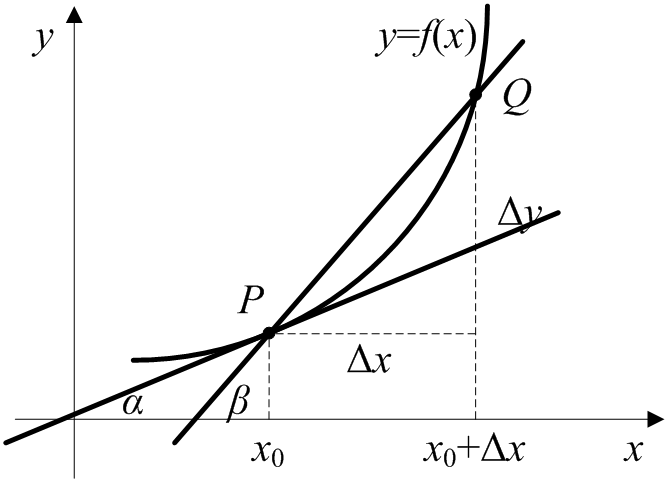
\includegraphics[height=4cm]{2.2.png}
\end{figure}

函数在{\it PQ}之间的变化率在几何上体现为割线{\it PQ}的斜率:
\[
\tan \beta =\frac{\Delta y}{\Delta x}
\]
函数在{\it P}点上的变化率在几何上体现为曲线在{\it P}点处的切线的斜率:
\[
\tan \alpha =\underset{\Delta x\rightarrow 0}{\lim}\frac{\Delta y}{\Delta x}=f'\left( x_0 \right)
\]
如果曲线沿着左右两个方向靠近{\it P}点时的切线斜率是一样的,就说明该点不折。
再看本章一开始的曲线,该曲线在$x_0$处左右导数都是有的,但不相等。
\begin{figure}[ht]
\centering
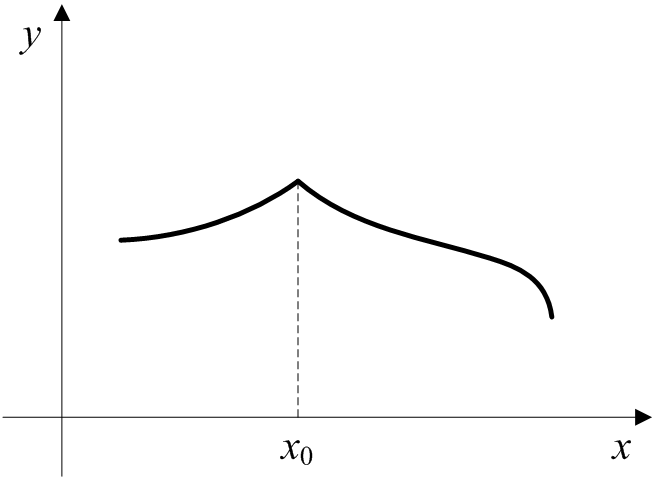
\includegraphics[height=4cm]{2.1.png}
\end{figure}

从几何上来讲,导数的意义是切线的斜率。
反映到光滑上,导数给出了对光滑的第二要求“不折”的数学定义。

%============================================================
\subsection{曲线的切线和法线}

我们将导数这个工具应用到曲线的分析上,分析曲线上任意一点处的切线和法线。

曲线在代数上可以定义为函数$y=f\left( x \right) ,x\in D$。现在我们已知曲线上任何一点$\left( x_0,y_0 \right) $处的斜率就是该点处的导数$f'\left( x_0 \right) $,于是我们得到了曲线上任意一点处的切线和法线的粗略的表达式:
\begin{align*}
&y_{tangent}=f'\left( x_0 \right) x+c \\
&y_{normal}=-\frac{1}{f'\left( x_0 \right)}x+c
\end{align*}
将点$\left( x_0,y_0 \right) $带入即可求得$c$,最终得到切线和法线方程如下:
\begin{align*}
&y_{tangent}=f'\left( x_0 \right) x+\left[ f\left( x_0 \right) -f'\left( x_0 \right) x_0 \right] \\
&y_{normal}=-\frac{1}{f'\left( x_0 \right)}x+\left[ f\left( x_0 \right) +\frac{1}{f'\left( x_0 \right)}x_0 \right]
\end{align*}

%============================================================
\subsection{导数的物理意义}

物理上,导数描述了一个物理量的瞬时变化速度。
比方说路程的导数是速度,速度的导数是加速度。
导数为求解物理量的变化速度提供了强大的数学工具。

有的时候,我们知道两个物理量之间的关系和其中一个物理量的变化率,通过导数就可以得到另一个物理量的变化率。
实际问题中,前者的变化率已知且简单,后者变化率复杂,无法直接获得,通过这个方法就可以获得一个复杂的、不直观的变化率。
换一种说法,我们要获得一个物理量的变化率,但该变化率复杂,难以通过常规的方法求解。
我们可以将它关联到一个具有简单已知的变化率的物理量,通过导数的运算和求导法则计算得到,比如观测仰角的变化率。

%============================================================
\subsection{导数的定理}

\begin{theorem}
$f\left( x \right) $在$x_0$处可导$\Leftrightarrow f\left( x \right) $在$x_0$处左右导数存在且相等,即$f'_-\left( x_0 \right) =f'_+\left( x_0 \right) $。
\end{theorem}

\begin{theorem}
$f\left( x \right) $在$x_0$处可导$\Leftrightarrow f\left( x \right) $在$x_0$处连续。
\end{theorem}

\begin{proof}
从连续的定义出发,即证明$\underset{x\rightarrow x_0}{\lim}\left[ f\left( x \right) -f\left( x_0 \right) \right] =0$。
\begin{align*}
\underset{x\rightarrow x_0}{\lim}\left[ f\left( x \right) -f\left( x_0 \right) \right] &=\underset{x\rightarrow x_0}{\lim}\frac{f\left( x \right) -f\left( x_0 \right)}{x-x_0}\cdot \left( x-x_0 \right) \\
&=f'\left( x_0 \right) \underset{x\rightarrow x_0}{\lim}\left( x-x_0 \right) =0
\end{align*}
\end{proof}

%============================================================
\subsection{导数的四则运算}

\begin{align*}
&\left( C\cdot f \right) '=C\cdot f' \\
&\left( f\pm g \right) '=f'\pm g' \\
&\left( f\cdot g \right) '=f'g+fg' \\
&\left( \frac{f}{g} \right) '=\frac{f'g-fg'}{g^2} \\
&\left( \frac{1}{g} \right) '=-\frac{g'}{g^2}
\end{align*}

前两个公式表明导数运算是线性的。

%============================================================
\subsection{导数的基本公式}

\begin{align*}
\begin{matrix}
	\left( C \right) '=0 \hfill                                       & \left( x^a \right) '=a\cdot x^{a-1} \hfill \\
	\left( a^x \right) '=a^x\ln a \hfill                              & \left( e^x \right) '=e^x \hfill \\
	\left( \log _ax \right) '=\frac{1}{x\ln a} \hfill                 & \left( \ln x \right) '=\frac{1}{x} \hfill \\
	\left( \sin x \right) '=\cos x \hfill                             & \left( \cos x \right) '=-\sin x \hfill \\
	\left( \tan x \right) '=\sec ^2x \hfill                           & \left( \cot x \right) '=-\csc ^2x \hfill \\
	\left( \sec x \right) '=\sec x\cdot \tan x \hfill                 & \left( \csc x \right) '=-\csc x\cdot \cot x \hfill \\
	\left( \mathrm{arc}\sin x \right) '=\frac{1}{\sqrt{1-x^2}} \hfill & \left( \mathrm{arc}\cos x \right) '=-\frac{1}{\sqrt{1-x^2}} \hfill \\
	\left( \mathrm{arc}\tan x \right) '=\frac{1}{1+x^2} \hfill        & \left( \mathrm{arc}\cot x \right) '=-\frac{1}{1+x^2} \hfill \\
	\left( \mathrm{sh}x \right) '=\mathrm{ch}x \hfill                 & \left( \mathrm{ch}x \right) '=\mathrm{sh}x \hfill \\
\end{matrix}
\end{align*}

以上基本公式中,除了$\left( C \right) ',\left( a^x \right) ',\left( \sin x \right) '$,其余都可以从这三个公式导出。

{\bf 计算$\left( C \right) '$}
\[
\left( C \right) '=\underset{\Delta x\rightarrow 0}{\lim}\frac{C-C}{\Delta x}=0
\]

{\bf 计算$\left( a^x \right) '$}
\[
\left( a^x \right) '=\underset{\Delta x\rightarrow 0}{\lim}\frac{a^{x+\Delta x}-a^x}{\Delta x}=a^x\underset{\Delta x\rightarrow 0}{\lim}\frac{a^{\Delta x}-1}{\Delta x}=a^x\ln a
\]

{\bf 计算$\left( \sin x \right) '$}
\begin{align*}
\left( \sin x \right) '&=\underset{\Delta x\rightarrow 0}{\lim}\frac{\sin \left( x+\Delta x \right) -\sin x}{\Delta x} \\
&=\underset{\Delta x\rightarrow 0}{\lim}\frac{2\sin \frac{\Delta x}{2}\cos \frac{2x+\Delta x}{2}}{\Delta x}=\underset{\Delta x\rightarrow 0}{\lim}cos \frac{2x+\Delta x}{2}=\cos x
\end{align*}

%============================================================
\subsection{复合函数的求导}

\begin{theorem}[复合函数求导定理]
若函数$y=y\left( u \right) ,u=u\left( x \right) $在对应区间可导,则复合函数$y=y\left[ u\left( x \right) \right] $在对应区间也可导,且有:
\[
\frac{dy}{dx}=\frac{dy}{du}\cdot \frac{du}{dx}
\]
\end{theorem}

复合求导法则是接下去三种求导法则(反函数求导、隐函数求导、参数式函数求导)的基础。

%============================================================
\subsection{反函数的求导}

\begin{theorem}[反函数求导定理]
若函数$y=f\left( x \right) $在某区间内单调可导,且$y'\ne 0$,则它的反函数$x=f^{-1}\left( y \right) $在对应区间内也可导,且有:
\[
f'\left( x \right) =\frac{1}{\left( f^{-1} \right) '\left( y \right)}
\]
或写成:
\[
\frac{dy}{dx}=\frac{1}{\frac{dx}{dy}}
\]
\end{theorem}

\begin{proof}
\[
f'\left( x \right) =\underset{\Delta x\rightarrow 0}{\lim}\frac{\Delta y}{\Delta x}=\underset{\Delta x\rightarrow 0}{\lim}\frac{1}{\frac{\Delta x}{\Delta y}}=\frac{1}{\underset{\Delta y\rightarrow 0}{\lim}\frac{\Delta x}{\Delta y}}=\frac{1}{\left( f^{-1} \right) '\left( y \right)}
\]
\end{proof}

~

\begin{example}
设$y=\mathrm{arc}\sin x$,求$y'$。
\end{example}

解:

\[
\frac{dy}{dx}=\frac{1}{\frac{dx}{dy}}=\frac{1}{\left( \sin y \right) '}=\frac{1}{\cos y}=\frac{1}{\sqrt{1-\sin ^2y}}=\frac{1}{\sqrt{1-x^2}}
\]

%============================================================
\subsection{隐函数的求导}

\begin{theorem}[一元隐函数求导定理]
若方程$F\left( x,y \right) =0$确定唯一的单值连续可导函数$y=f\left( x \right) $,则有:
\[
\frac{dy}{dx}=-\frac{F_x}{F_y}
\]
其中:
\begin{itemize}
	\item $F_x$:表示$F\left( x,y \right) =0$对$x$求导,$x$是自变量,$y$是常量;
	\item $F_y$:表示$F\left( x,y \right) =0$对$y$求导,$y$是自变量,$x$是常量。
\end{itemize}
\end{theorem}


\begin{tcolorbox}
该定理在多元函数微积分中证明,这里只需知道如何计算一元隐函数的导数。
\end{tcolorbox}

~

\begin{example}
假设方程$e^y=e-xy$确定了函数$y=f\left( x \right) $,求$y'$。
\end{example}

解:

令$F\left( x,y \right) :=e^y-e+xy=0$,得:
\begin{align*}
&\because \begin{cases}
	F_x=y\\
	F_y=e^y+x\\
\end{cases} \\
&\therefore y'=-\frac{F_x}{F_y}=-\frac{y}{e^y+x}
\end{align*}

%============================================================
\subsection{参数式函数的求导}

\begin{theorem}[参数函数求导定理]
若参数方程
\begin{align*}
\begin{cases}
	x=x\left( t \right)\\
	y=y\left( t \right)\\
\end{cases}
\end{align*}
可导,$x=x\left( t \right) $存在可导的反函数,且$x'\left( t \right) \ne 0$,则由该参数方程确定的函数$y=f\left( x \right) $可导,且有:
\[
\frac{dy}{dx}=\frac{y'\left( t \right)}{x'\left( t \right)}
\]
\end{theorem}

~

\begin{example}
若有摆线
\begin{align*}
\begin{cases}
	x=t-\sin t\\
	y=1-\cos t\\
\end{cases}
\end{align*}
求$t=\pi /2$处的切线方程。
\end{example}

解:

切线方程$y=f'\left( x_0 \right) x+\left[ f\left( x_0 \right) -f'\left( x_0 \right) x_0 \right] $,可得:
\begin{align*}
&\left. \frac{dy}{dx} \right|_{t=\pi /2}=\left. \frac{dy}{dt}/\frac{dx}{dt} \right|_{t=\pi /2}=\left. \frac{\sin t}{1-\cos t} \right|_{t=\pi /2}=1 \\
&y=1\cdot x+\left[ \left( 1-\cos \frac{\pi}{2} \right) -1\cdot \left( \frac{\pi}{2}-1 \right) \right] =x+2-\frac{\pi}{2}
\end{align*}

%============================================================
\subsection{高阶导数}

\begin{definition}[二阶导数]
设函数$f\left( x \right) $在点$x_0$的某邻域$N\left( x_0 \right) $内可导,若极限
\[
\underset{\Delta x\rightarrow 0}{\lim}\frac{f'\left( x_0+\Delta x \right) -f'\left( x_0 \right)}{\Delta x}
\]
存在,则称该极限值为{\bf $f\left( x \right) $在点$x_0$处的二阶导数},记作:
\[
f''\left( x_0 \right) \quad \text{或} \quad \left. y'' \right|_{x=x_0} \quad \text{或} \quad \left. \frac{d^2y}{dx^2} \right|_{x=x_0}
\]
\end{definition}

同样,我们可以定义三阶导数、四阶导数、直至n阶导数。




